\newpage
\chapter{Arquitectura del Clúster}
\label{ch:capitulo2.tex}

\begin{FraseCelebre}
	\begin{Frase}
		Bueno, pero aparte del alcantarillado, la sanidad, la enseñanza, el vino, el orden público, la irrigación, las carreteras y los baños públicos, ¿qué han hecho los romanos por nosotros?
	\end{Frase}
	\begin{Fuente}
	The Life Of Brian
	\end{Fuente}
\end{FraseCelebre}

A lo largo de este capitulo hablaremos de cada uno de los elementos que componen el cluster, detallando alguna de sus características mas importantes y evaluando los problemas derivados de estas.

\section{Componentes}
\label{makereference2.1}

Cada uno de los componentes que se describen a continuación fueron obtenidos a través del Proyecto de Innovación Docente de la Universidad Complutense y formarán parte del material accesible a los alumnos de la asignatura de Programación de Sistemas Distribuidos. Uno de los objetivos finales del proyecto es el de permitir a futuros alumnos de la asignatura una plataforma para el desarrollo de las prácticas de la misma, así como un modelo real con el que poder afianzar conocimientos sobre clusteres y grandes sistemas de computación. Con el presupuesto obtenido para este proyecto, aproximadamente setecientos cincuenta euros, hemos obtenido material suficiente para el montaje final.

\subsection{Raspberry Pi Modelo B}

Hemos elegido Raspberry Pi como nodo de cómputo debido a su limitado consumo, tamaño reducido y bajo coste. Las características de ésta, que resumimos a continuación, hacen que sea perfecta para el diseño de proyectos de diversos tipos y, como hemos expuesto en el capítulo anterior, existe una gran variedad de proyectos desarrollados para ella. 

\subsubsection{}

\begin{figure}[H]
	\centering
  	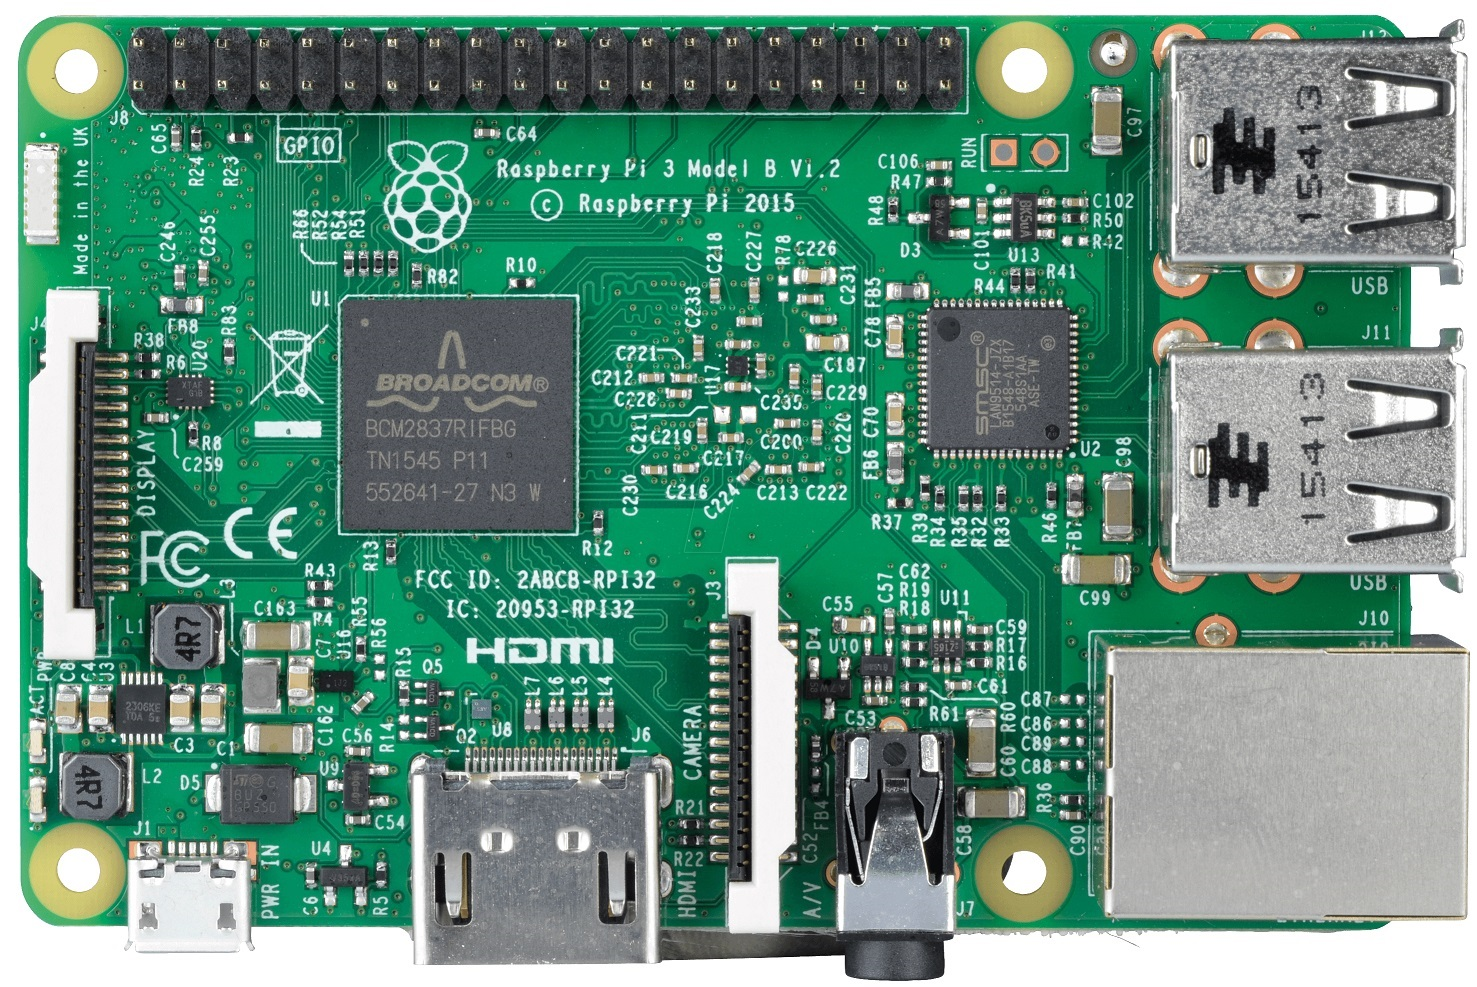
\includegraphics[width=50mm]{pics/rpi3b.jpg}
   	\caption[Raspberry Pi Modelo 3 b]{Raspberry Pi Modelo 3 b}
   \label{figure2.1}
\end{figure}

\subsubsection{}


\subsubsection{Especificaciones}

\begin{itemize}
  \item Chipset Broadcom BCM2387
  \item 1,2 GHz de cuatro núcleos ARM Cortex-A53
  \item 1 GB LPDDR2
  \item Ethernet socket Ethernet 10/100 BaseT
  \item 802.11 LAN inalámbrica
  \item HDMI rev 1.3 y 1.4
  \item USB 4x Conector USB 2.0
  \item Conector GPIO
\end{itemize}

\subsubsection{Límites térmicos}

Uno de los mayores problemas de utilizar Raspberry Pi para el proyecto es que crecen de elementos de disipación de calor propios integrados en la placa, lo que hace que sea especialmente sensible a las altas temperaturas. Bajo una situación de poco estrés mantiene unos rangos de temperatura bastánte estables, sobre los cuarenta grados ºC, pero bajo condiciones de mucha carga de trabajo el aumento de la temperatura es bastánte elevado, llegando a su punto crítico sobre temperaturas cercanas a los ochenta grados ºC, condiciones en las cuales, por seguridad, se produce un apagado súbito del sistema. En la figura \ref{figure2.8} se puede apreciar un procesador con sobre la temperatura crítica de apagado.

\begin{figure}[H]
	\centering
  	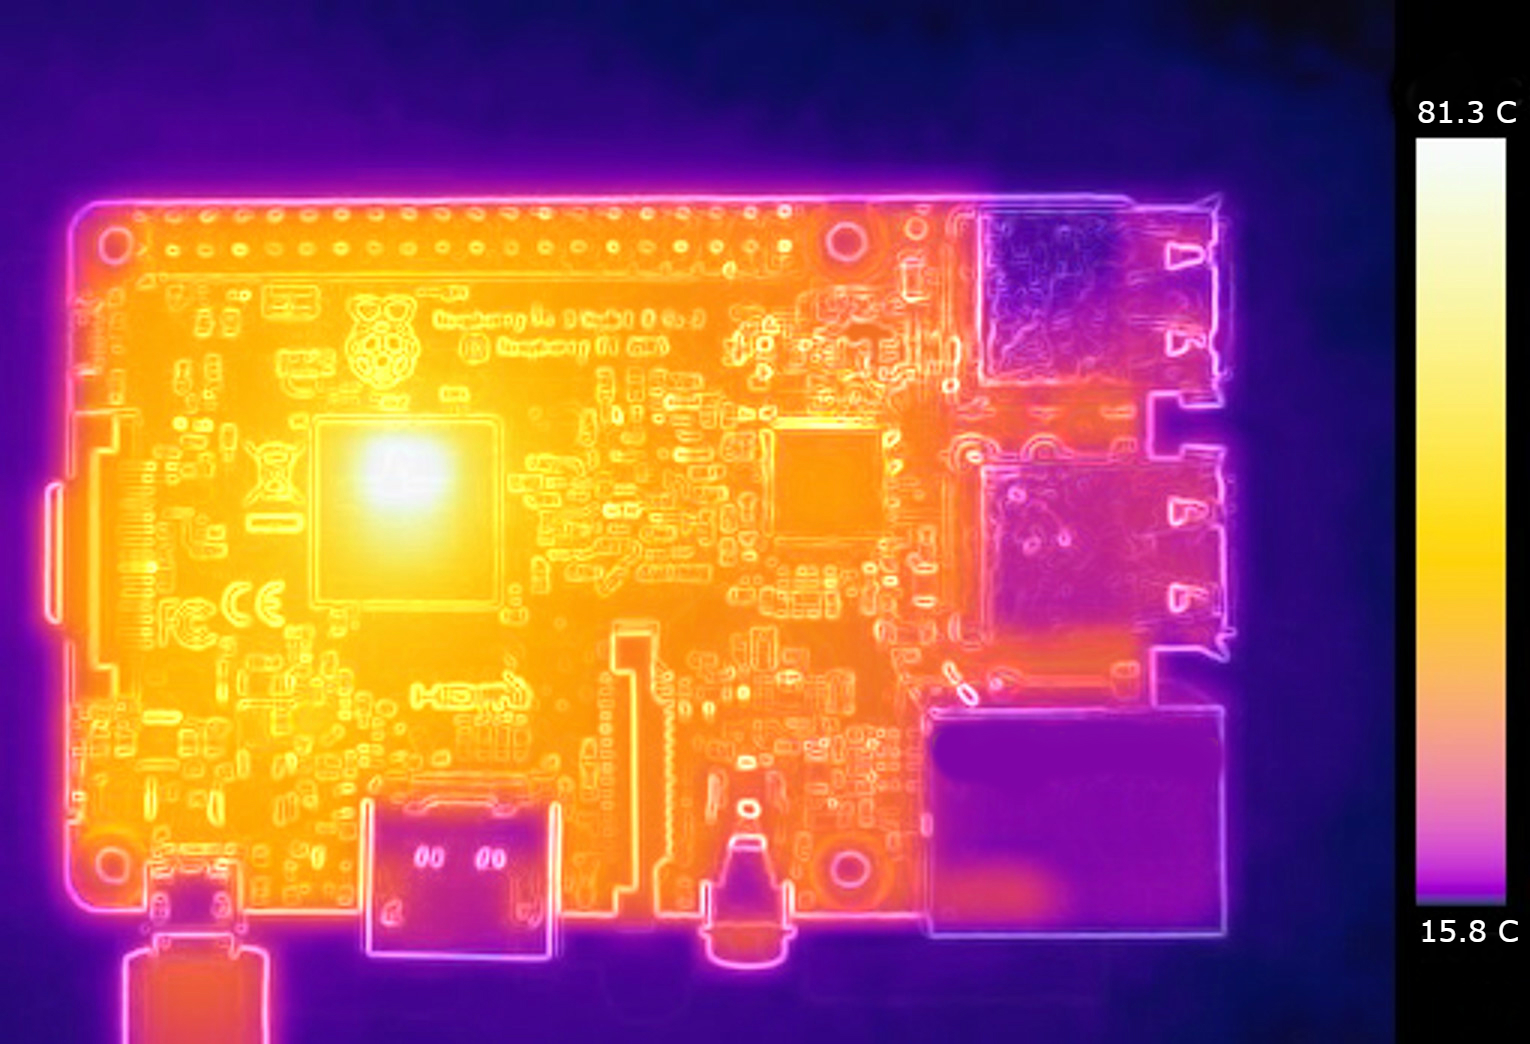
\includegraphics[width=60mm]{pics/pi_3_thermal.jpg}
   	\caption[Captura Térmica]{Límite térmico de la Raspberry}
   \label{figure2.8}
\end{figure}

Esto afecta principalmente a la memoria, controlador de Ethernet y los procesadores.

Debido a la disposición de las tarjetas en forma de columna, existe una gran proximidad entre ellas, lo que hace que aquellas que se encuentren el las partes mas centrales de la estructura estén expuestas a un efecto de tubo de calor proviniente de los nodos que se encuentran próximos a ellas, por esto es necesario disponer de un buen método de disipación de calor, a fin de evitar el sobrecalentamiento del sistema. La disposición y soluciones aportadas a este problema se describen mas ampliamente en el capítulo \ref{ch:capitulo4.tex}.

\subsubsection{Disipadores de calor}

Una de las soluciones aportadas para resolver el problema que se acaba de describir es incluir disipadores de calor sobre el procesador, memoria y controlador Ethernet.

\begin{figure}[H]
	\centering
  	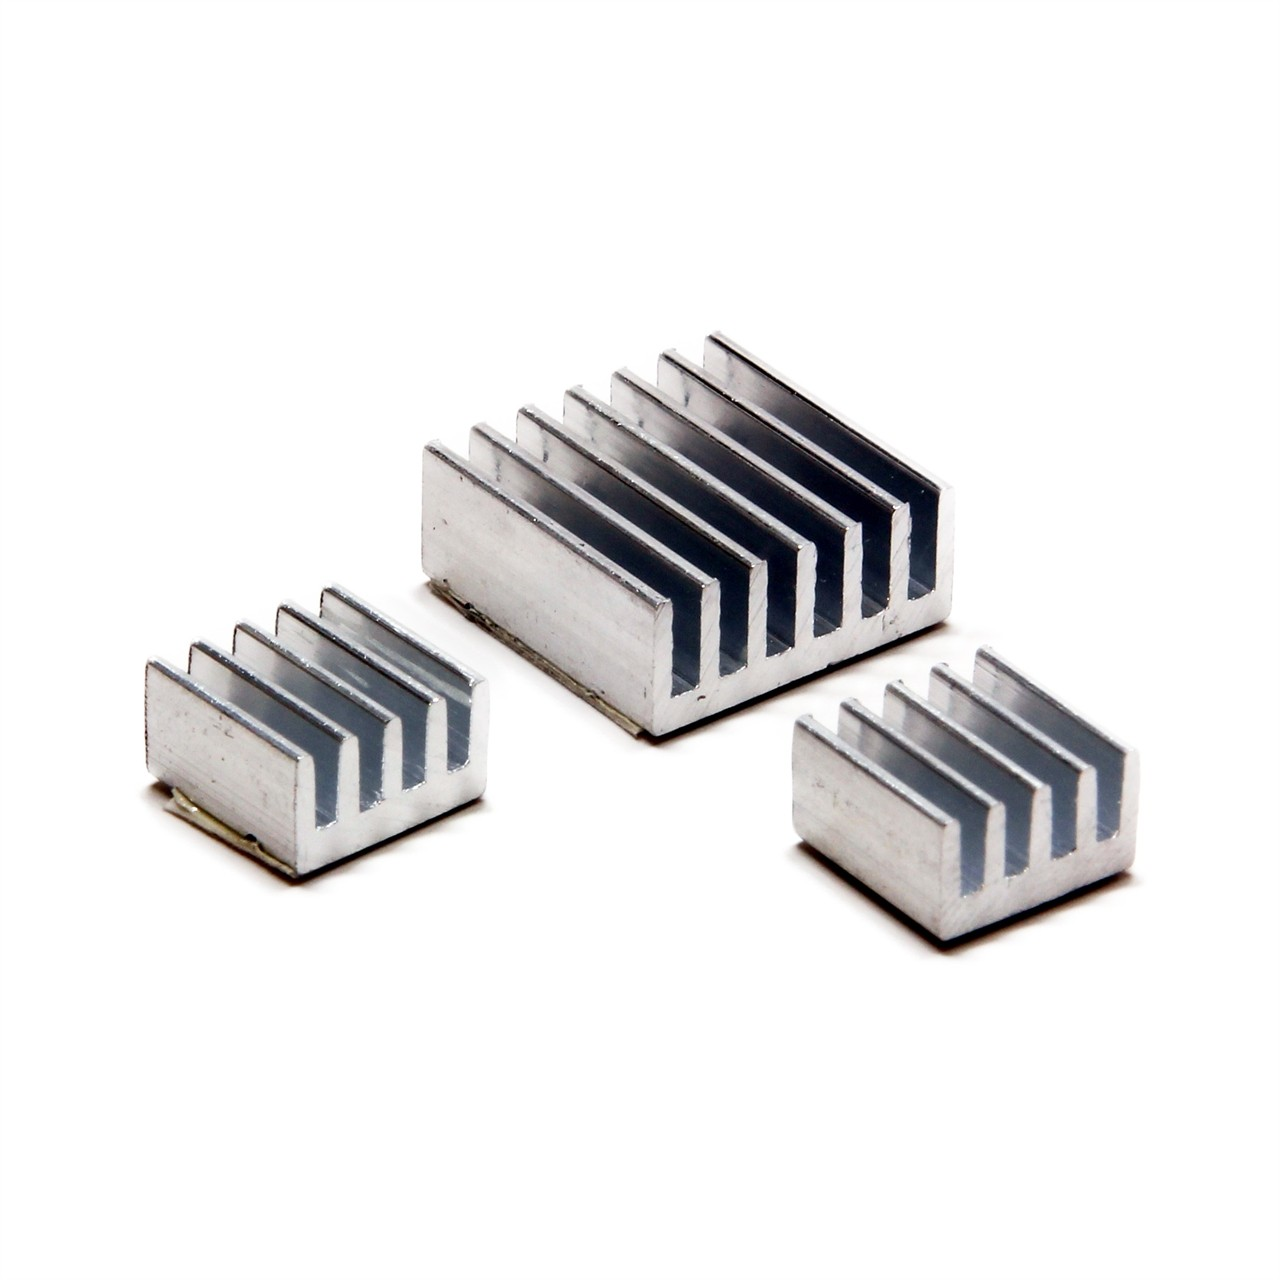
\includegraphics[width=50mm]{pics/disipadores.jpg}
   	\caption[Disipadores ]{Disipadores}
   \label{figure2.8}
\end{figure}

Estos tiene un precio muy reducido y como veremos más adelante, aunque por si solos no suponen una gran mejora, aproximadamente unos dos o tres grados ºC menos que un nodo que no disponga de ellos, con una buena ventilación ofrecen una mejora realmente notoria.

\subsection{Conversor USB 3.0 a Ethernet}

Raspberry 3 modelo B sólo posee un puerto Ethernet, nuestro nodo maestro necesita disponer de un puerto dedicado para cada una de sus conexiones con el front-end y el back-end. Ete dispositivo permite ampliar el número de puertos Ethernet para solucionar dicho problema 

\begin{figure}[H]
	\centering
  	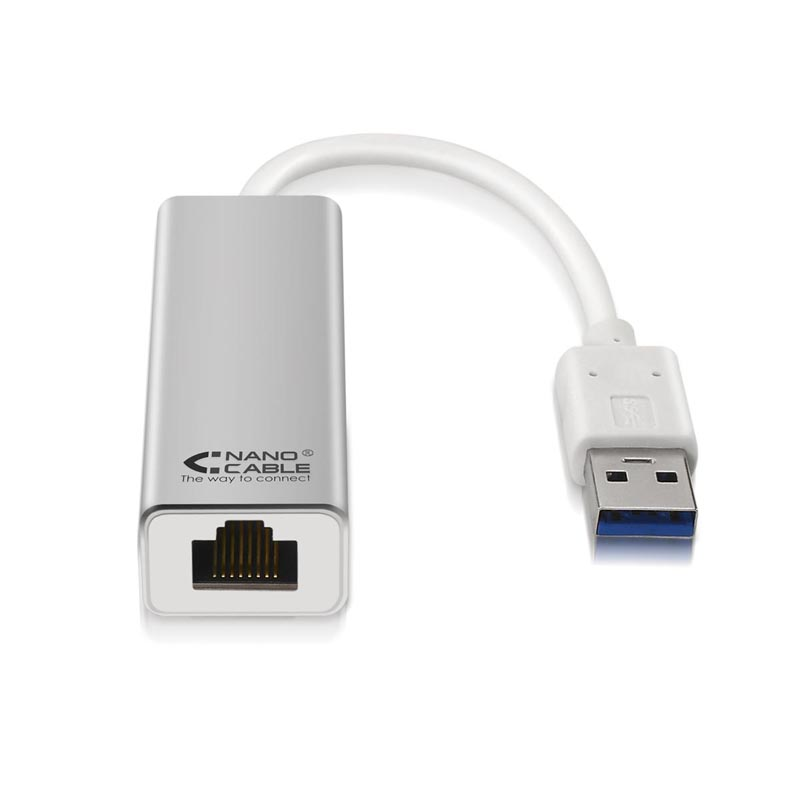
\includegraphics[width=60mm]{pics/ethernetUSB.jpg}
   	\caption[Conversor USB 3.0 a Ethernet]{Conversor USB 3.0 a Ethernet}
   \label{figure2.3}
\end{figure}

\subsubsection{Especificaciones}

\begin{itemize}
  \item Conexión USB 3.0
  \item Compatible con IEEE 802.3, 802.3u y 802.3ab
  \item Chipset RTL8153
  \item Velocidad de transferencia de datos: 10, 100, 1000 Mbps
  \item Detección de crossover y corrección automática
\end{itemize}

Uno de los factores destacables de este componente es que sí puede alcanzar una tasa de transferencia de 1000 Mbps, a diferencia del puerto Ethernet instalado en la Raspberry Pi, esto permite disponer de una mayor velocidad de cara al front-end, permitiendo unas comunicaciones mas fluidas con el exterior del cluster. 

\subsection{Tarjeta microSD SanDisk}

Raspberry Pi no dispone de almacenamiento en disco, en vez de eso dispone de una ranura microSD en la cual viene instalado el sistema operativo. La capacidad de las tarjetas es un factor importante a tener en cuenta ya que la instalación del sistema operativo en tarjetas de un tamaño superior a los 32 Gigabytes requiere de un software específico, haciendo que la instalación sea mas compleja y, como hemos podido comprobar, no es soportada por todas las versiones de Debian Jessie disponibles en el repositorio oficial de raspberypi.org.

\begin{figure}[H]
	\centering
  	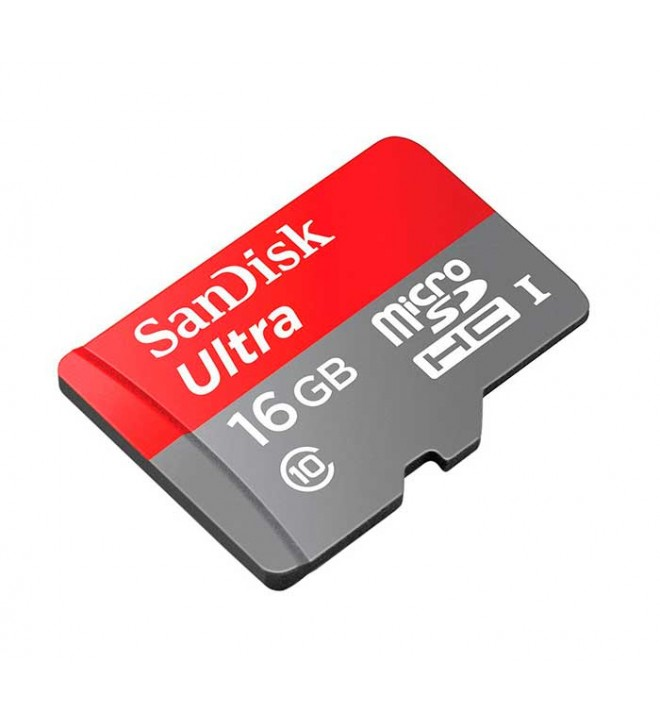
\includegraphics[width=40mm]{pics/sd.jpg}
   	\caption[microSD SanDisk]{microSD SanDisk}
   \label{figure2.2}
\end{figure}

Debido a que el sistema al completo no supera los 11 Gigabytes tanto en los nodos esclavos como en el maestro decidimos usar tarjetas de 16 Gigabytes para todos los nodos de la red, de esta forma reducimos se reduce el gasto y evitamos problemas de compatibilidad entre algunas versiones de Debian Jessie.

\subsection{Switch D-LINK DGS-1008D}

La elección del switch es importante ya que limita el número de nodos que puede haber dentro del cluster, esto, junto con los  cables de alimentación, tiene una influencia directa sobre el tamaño del contenedor, así como la escalabilidad del cluster. Por otro lado, el reducido presupuesto no nos ha permitido disponer de más nodos de cómputo, debido a todos estos parámetros decidimos trabajar con un switch de ocho puertos, lo que permite disponer de hasta siete nodos de cómputo, ya que una de las entradas del mismo sirve como puente entre módulos, permitiendo, en caso de que se requiera, aumentar el número de nodos.

\begin{figure}[H]
	\centering
  	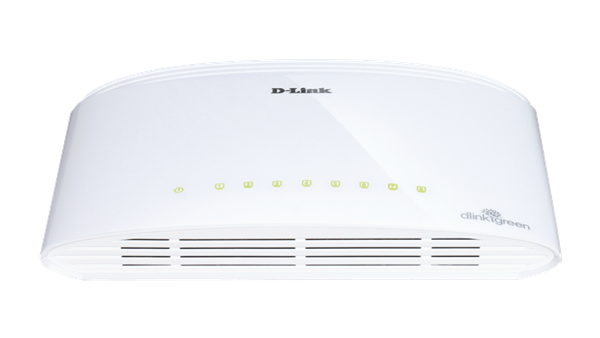
\includegraphics[width=60mm]{pics/DGS_1008DSwitch8.png}
   	\caption[Switch D-LINK DGS-1008D]{Switch D-LINK DGS-1008D}
   \label{figure2.2}
\end{figure}

\subsubsection{Especificaciones}

\begin{itemize}
  \item 8 Puertos Ethernet 1000/100/10 Mbps
  \item Velocidad de transferencia: 2000 Mbps full duplex
\end{itemize}

Como podemos ver en las especificaciones este modelo permite alcanzar una velocidad de hasta 1000 Mbps, sin embargo el modelo de Raspberry Pi utilizado está limitado a 100 Mbps. En la versión mas reciente de Raspberry (Modelo B+), este límite sigue vigente, sin embargo se espera que posteriores modelos alcancen esta velocidad, lo que mejoraría las comunicaciones dentro del equipo. 



\subsection{Ventiladores}
\subsubsection{Especificaciones}

\begin{figure}[H]
	\centering
  	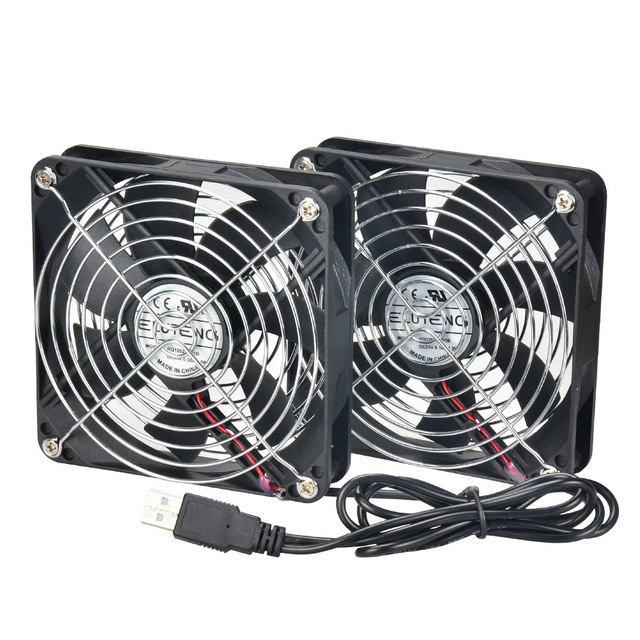
\includegraphics[width=60mm]{pics/fan120.png}
   	\caption[Ventiladores USB]{Ventiladores USB}
   \label{figure2.4}
\end{figure}

\subsection{Cargador USB}

\subsubsection{Especificaciones}
\begin{figure}[H]
	\centering
  	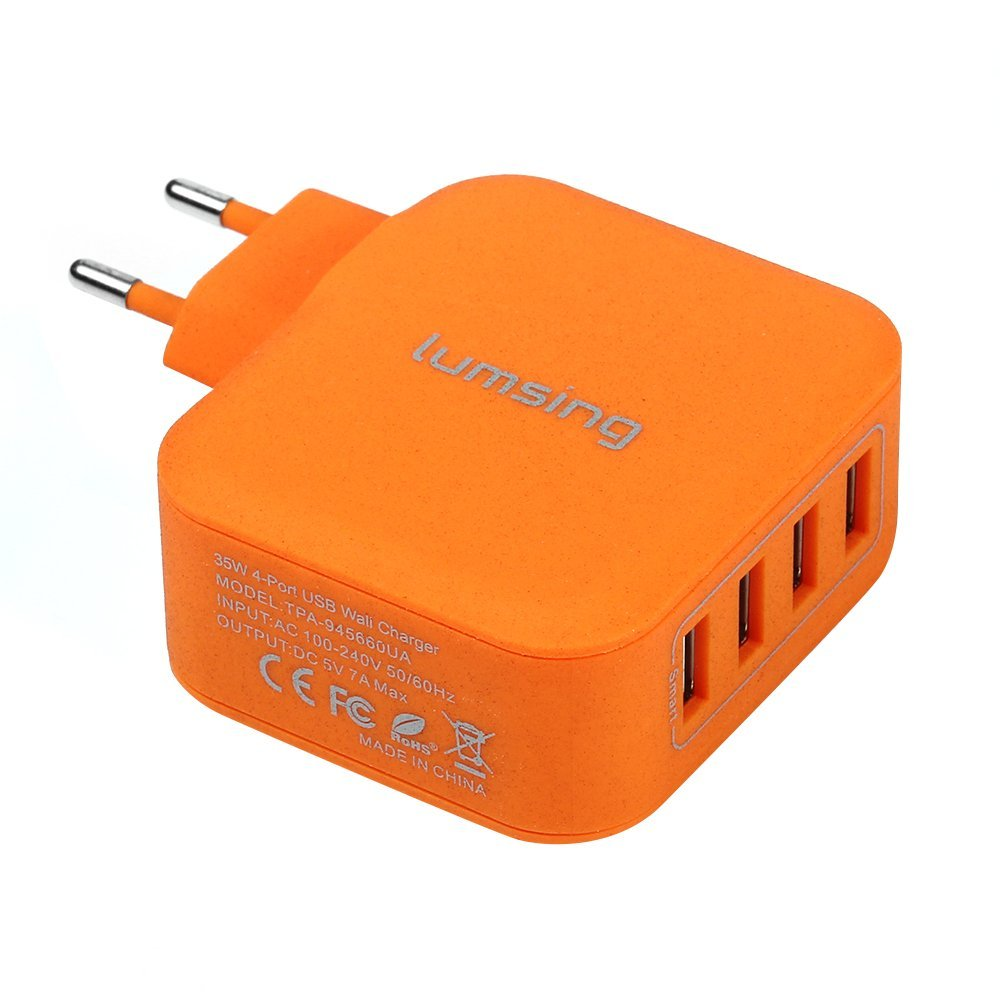
\includegraphics[width=60mm]{pics/cargadorUSB.jpg}
   	\caption[Cargador USB]{Cargador USB}
   \label{figure2.5}
\end{figure}

\subsubsection{Falta de energía}

La raspberry necesita de tres Amperios para poder funcionar, inicialmente el encargado de alimentar al cluster era un Hub de 10 puertos como el de la figura \ref{figure2.7}, tras las primeras pruebas descubrimos que repartía de forma uniforme la energía a todo el sistema y no conseguía llegar a satisfacer(sí, he dicho satisfacer) a ninguna raspberry por separado.//REVISAR


\begin{figure}[H]
	\centering
  	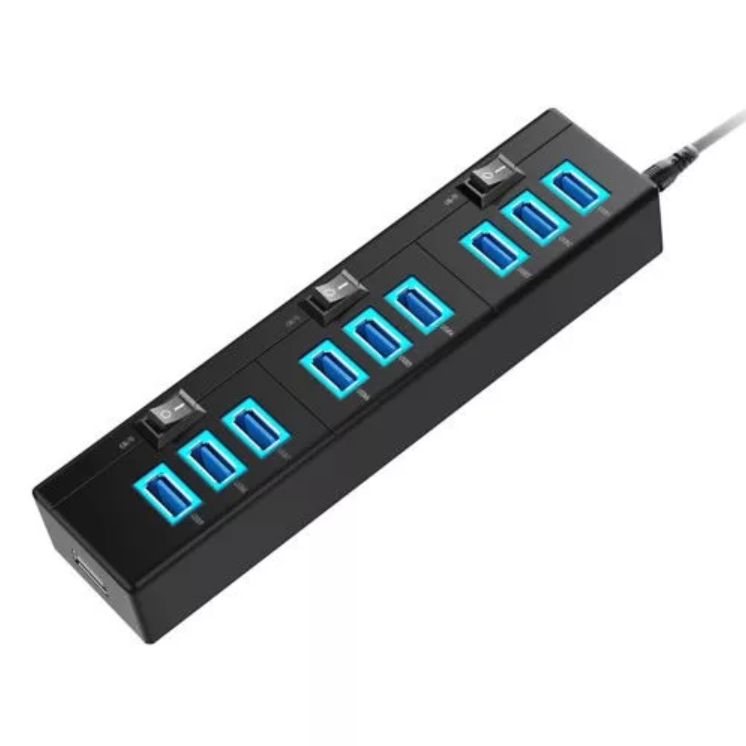
\includegraphics[width=60mm]{pics/Hub.PNG}
   	\caption[Problemas de energía]{Hub Inicial}
   \label{figure2.7}
\end{figure}


La solución a este problema la hallamos en dos cargadores como los de la figura \ref{figure2.5} de cuatro puertos y que reparten de forma eficiente alimentación a tres raspberrys y un ventilador cada uno.